\documentclass[11pt,a4paper]{report}

\usepackage[utf8]{inputenc}
\usepackage[french]{babel}
\usepackage{graphicx}

\author{Benjamin Pajusco et Paul ALNET}
\title{Systèmes électoraux: enjeux et  emplois au sein des démocraties}
\date{2020}

% Pour citer sans que cela n'aparaisse on utilise \nocite{bibid}
% On pourra éventuellement les changer automatiquement en \cite

% For the title background, via https://tex.stackexchange.com/questions/46280/how-to-create-a-background-image-on-title-page-with-latex
\usepackage{eso-pic}
\newcommand\BackgroundPic{%
	\put(0,-180){%
		\parbox[b][\paperheight]{\paperwidth}{%
			\vfill
			\centering
			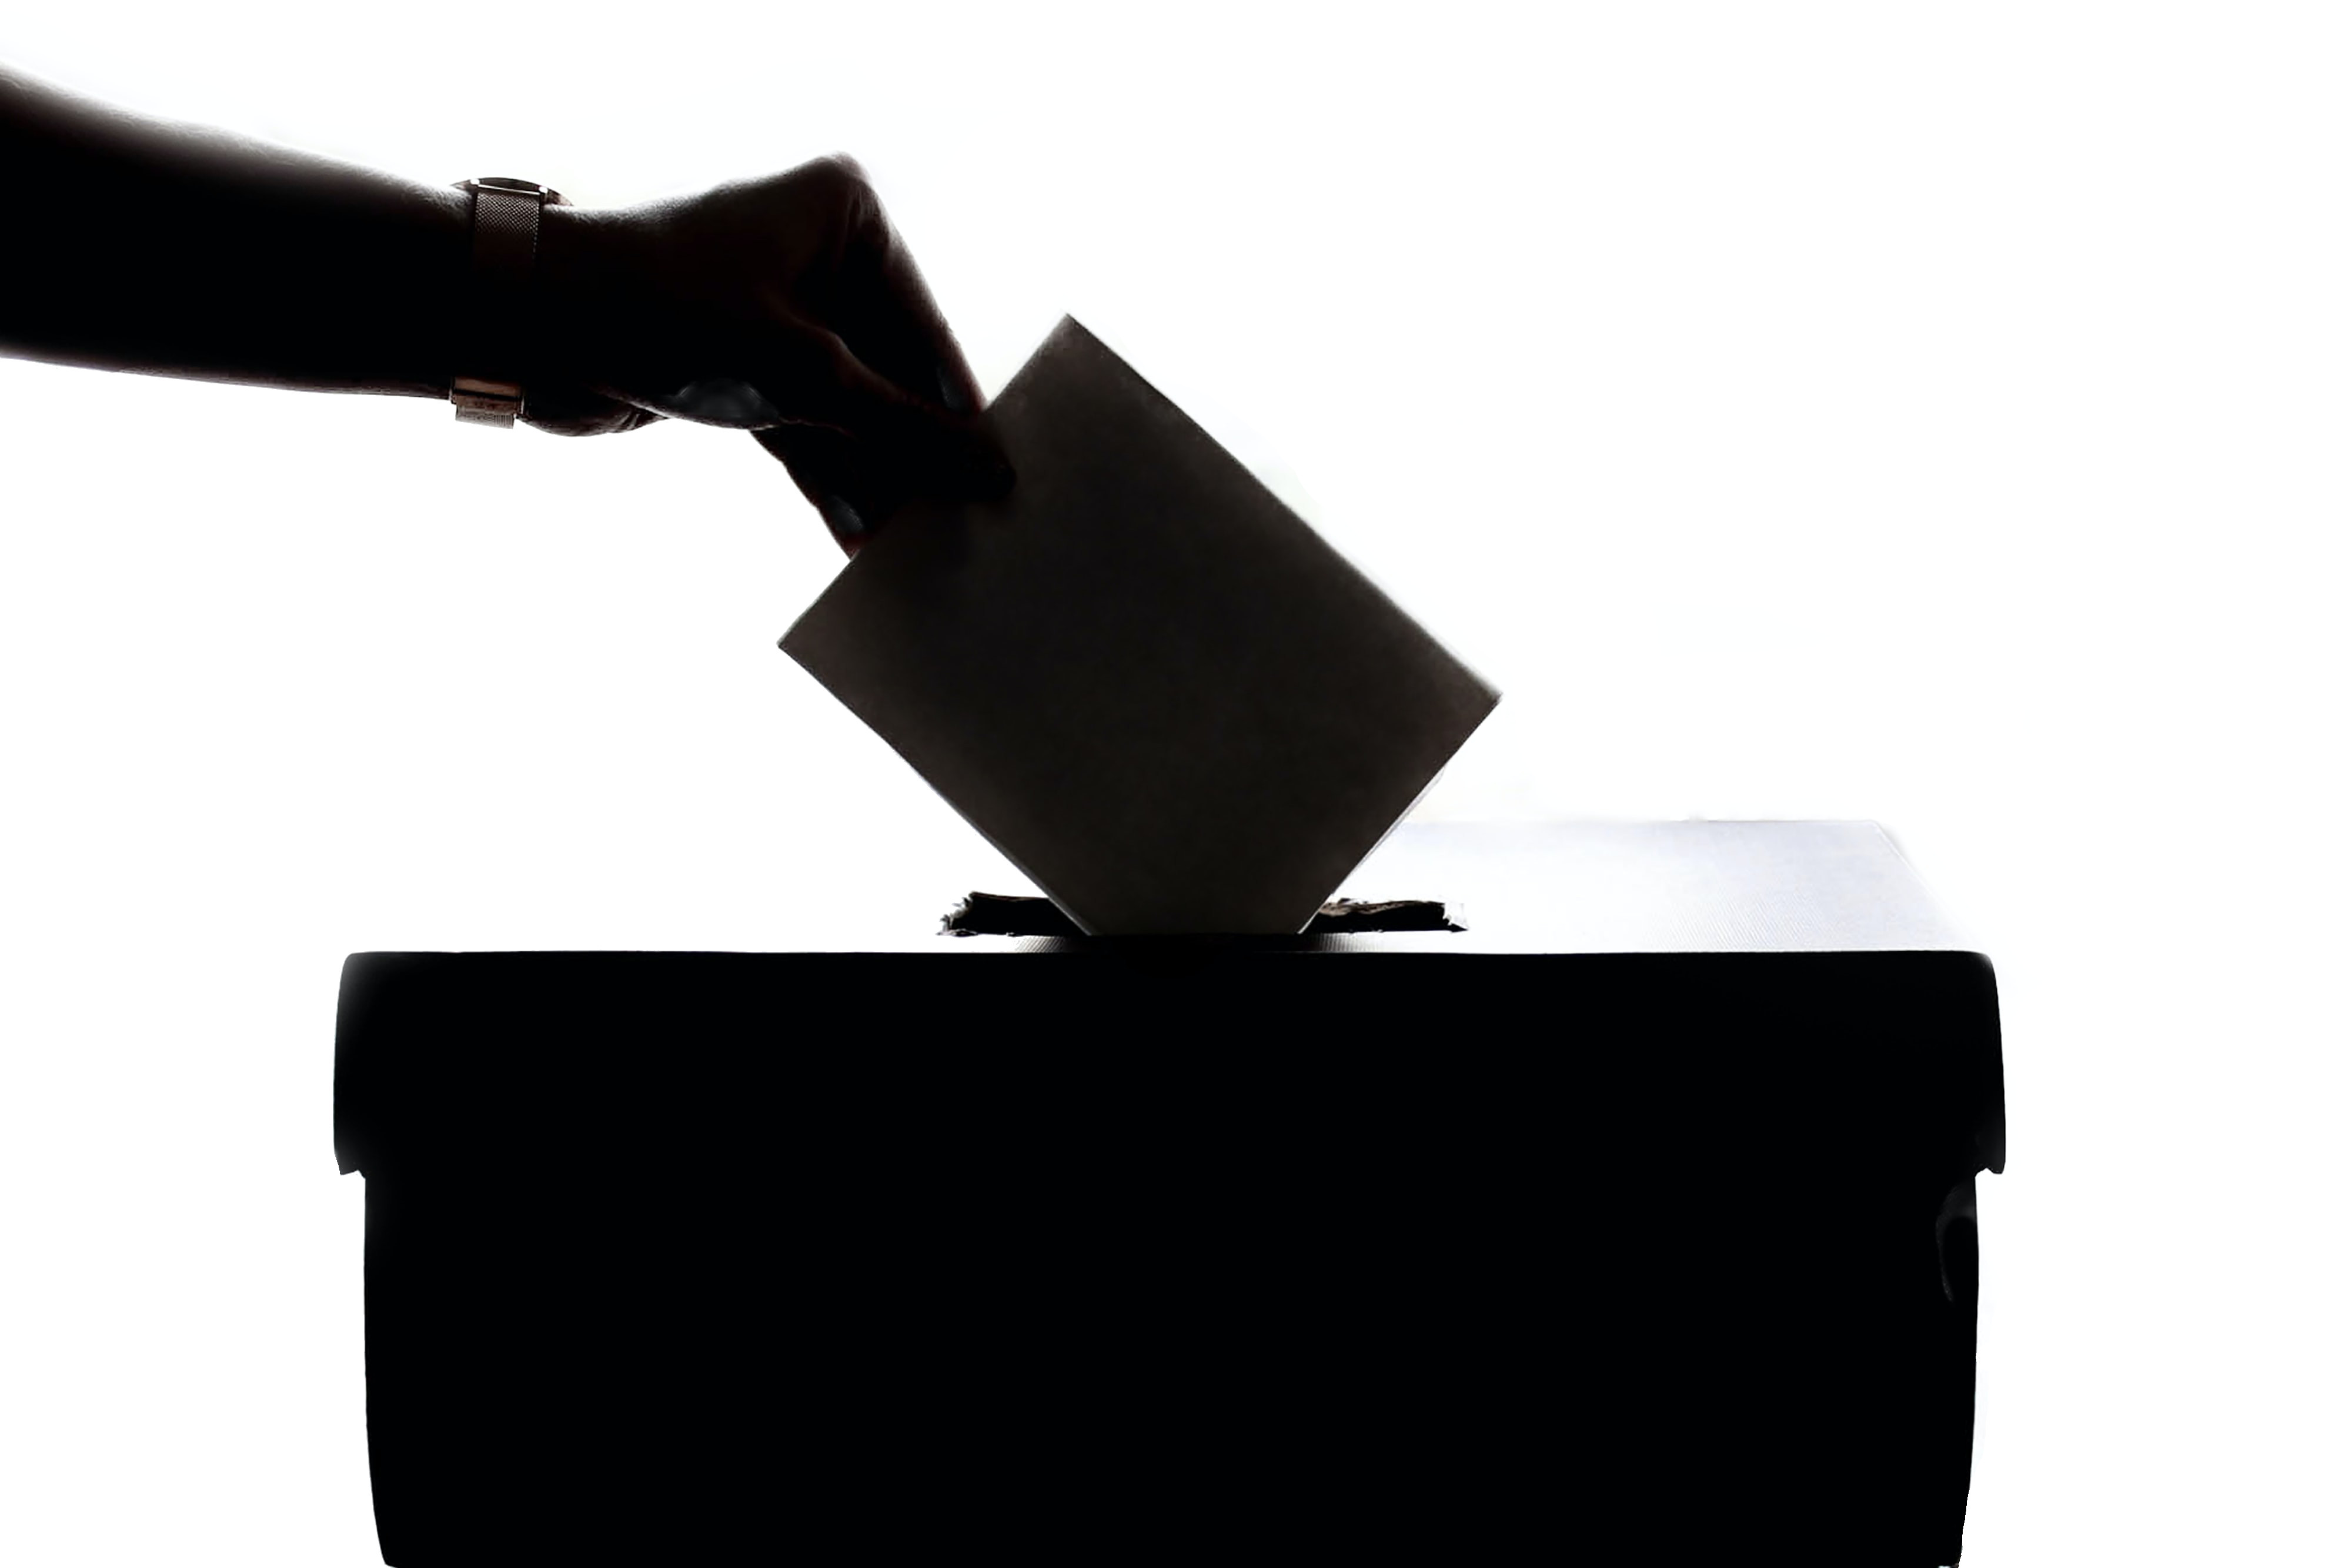
\includegraphics[width=\paperwidth,height=\paperheight,%
			keepaspectratio]{background.jpg}%
			\vfill
			
}}
	\put(100,36){\tiny{Photo par @element5digital sur Unsplash, légèrement altérée}}
}

\begin{document}
\AddToShipoutPicture*{\BackgroundPic}
\maketitle

\textbf{Quelles sont les différentes approches pour donner la voix au peuple, leurs évolutions et quelles sont les conséquences de leurs implémentations?}

\section*{Introduction}
 L'avenant des gouvernements, la transition progressive vers des états plus démocratiques, le pouvoir théoriquement donné au au peuple, nécessite l'apport d'une méthode pour permettre à chaque citoyen de faire entendre sa voix, son opinion. \nocite{wiki:demo}
 Chacun devant vaquer à ses occupations et ne pouvant pas investir temps et ressources dans la vie démocratique ainsi que la soif accrue du pouvoir détenue par certains font que l'on opte plutôt pour désigner des représentants du peuple, souvent par le biais d'élections; on appelle ceci la démocratie représentative. \nocite{wiki:seppv}
 Aristote déjà conçoit que celle-ci doit s'accompagner d'une séparation des pouvoirs. C'est à dire que les pouvoirs législatif, qui établit la loi et le budget de l'État, exécutif, qui applique la loi, et judiciaire, qui veille à la bonne application de la loi, sont partagés par différents groupes d'individus, au contraire d'une autocratie. \nocite{viepub:seppv}
 
 Ces personnes n'apparaissent pas magiquement, des procédés, variant selon les pays et régions, sont dictés dans les lois et sont suivis pour déterminer qui représentera, qui dirigera la nation.
 Nombreuses sont les organisations plaçant à la tête du pouvoir exécutif une hiérarchie menée par une personne élue, souvent président ou premier ministre, nommant les autres membres de la tête de l'administration. Il est généralement admis que cette personne dirigeante devrait être élue par le peuple, démocratiquement. 
 Ce défi logistique est confronté avec diverses approches selon les pays.
 
   Les modèles des démocraties modernes ne sont pas apparues instantanément mais découlent de plus de deux millénaires d'évolution.

TODO peaufiner

\tableofcontents

\nocite{wiki:histdemo}
\chapter{Majorité simple}
Il s'agit d'une méthode très simple de rendre compte de l'avis des électeurs pour répondre à une question binaire, bien que l'on puisse parfois s'abstenir.
On comptabilise le nombre de votants en faveur du premier choix, si cette valeur est supérieure à la moitié du nombre de votants, ce choix rentre en vigueur.


TODO Referendum en France
\section{Démocratie Athénienne}
La capitale de la Grèce antique Athènes est reconnue comme l'une des premières origines de démocratie. 
En effet, au VI\up{e} siècle avant notre ère, la cité est, comme tant d'autres, confrontée à une crise politique. 
Pour y pallier, les législateurs renforcent le caractère démocratique du régime et rendent plus accessible la politique aux citoyens moins aisés en proposant notamment des compensations monétaires.

\subsection{Le corps électoral}
Si l'agglomération athénienne comptait 250 000 habitants\nocite{persee:popu}, seuls les citoyens peuvent voter. 
Or les femmes et esclaves n'étaient considérés que comme mineurs, seuls les fils de citoyen ayant suivi l'équivalent du service militaire moderne peuvent jouir du titre de citoyen.
 
Ces restrictions laissent un corps de 40 000 citoyens, composé de 


\chapter{Scrutin uninominal majoritaire à deux tours}
TODO Fr

\chapter{Suffrage indirect}
Ce système d'élection est particularisé par la présence d'intermédiaires entre les électeurs du peuple et les concurrents. 
C'est à dire que les citoyens votent non pas directement pour les candidats mais plutôt pour des "grands électeurs" qui eux choisiront ultimement qui obtiendra le pouvoir.
Cette organisation, initialement préférée dans les jeunes démocraties, permettant de maintenir au pouvoir des personnes moins populaires mais aimées de ceux déjà en haut au détriment du peuple peu informé, perd progressivement en réputation avec l'éducation des citoyens et l'accessibilité croissante à l'information.
\nocite{wiki:scrutinindir}

La V\up{ème} République a employé cette méthode de suffrage pendant sa première élection, avant que le \textit{referendum} proposé par Charles De Gaulle ne soit validé et un suffrage direct établi.

\section{Implémentation aux États-Unis}
TODO intro
\nocite{wiki:eleccoll}
TODO peaufiner \& faire paragraphes

\subsection{Éligibilité et Historique}
Tout d’abord, il y a des prérequis afin d’être président des États-Unis.
Il faut être minimum âgé de 35 ans, être citoyen des États-Unis à sa naissance, avoir résidé aux États-Unis plus de 14 ans et ne pas être à son troisième mandat.
Ces dernières années, deux partis sont principalement représentés, le parti démocrate et le parti republicain.

Les élections présidentielles durent dans ce pays depuis 1789.
Cependant les lois furent un petit peu changées en 1803 mais le modèle utilisé actuellement est celui avec les lois changé en 2009.
Les changement de lois sont internes aux états donc le système de vote est le même, la constitution n'a elle pas changé.
Un point historique important est aussi la fixation du “Election day” étant le premier mardi du mois de novembre.
C’est le jour fixé par la loi pour l'élection du suffrage universel.

\subsection{Fonctionnement}
Le modèle de vote pour les élections présidentielles aux états unis est basé sur un scrutin dit “indirect”.
Ce modèle de vote est un système d'élection ou les électeurs ne choisissent pas eux même la personne qui va être élue mais ils élisent des personnes qui vont faire ce choix.
Dans le cadre des États-Unis, chaque État possède un certain nombre d'électeurs.
Ces électeurs sont comptés au nombre de 538 répartis entre chaque État.
Prenons pour exemple l'État d'Ohio qui possède 18 grands-électeurs.
Si le vote des citoyens et majoritairement pour le parti démocrate.
Le parti démocrate empoche alors 18 votes car il y a la politique du “winner takes all” qui explique que la majorité des votes emporte l'entièreté des grands électeurs d’un état.
Ceci dit, il n’est pas non plus interdit qu’un grand électeur vote pour autre chose que la majorité choisie par les citoyens, mais il risque de grosses amendes pour candidat déloyal dans la majorité des états.
Pour gagner les élections présidentielles américaines, il faut que le candidat obtienne plus de 270 votes de la part des grands électeurs.
Si jamais la majorité absolue n’est pas atteinte par l’un des deux candidats, c’est alors la Chambre des représentants qui élit le président et le Sénat qui désigne le Vice-président.
\nocite{wiki:electday}
\nocite{wiki:elecus}

\subsection{Avantages / Désavantages}
Ce système de vote montre des avantages et des inconvénients.
Un avantage est la Représentation régionale plus équitable.
On donne ici une force plus ou moins équitable à chaque Etat, petit ou grand.
Le problème de cet avantage est aussi un inconvénient.
Si un petit État possède une force plus ou moins égale à celle dans un plus grand État, chaque habitant ne possède pas le même impact sur l'élection du président.
La voix d’un habitant d’un tout petit état vaudra alors beaucoup plus que quelqu’un dans un grand état.
Cela apporte donc un nouveau désavantage qui est qu’un candidat peut passer à la tête d’un pays alors qu’il ne possède pas la majorité du vote populaire, ce qui s’est produit en 1824, 1876, 1888, 2000 et 2016.
Un autre avantage de ce système est le résultat.
Si jamais il y a des problèmes de fraudes en termes de votes ou quoi que ce soit en termes de doute, il n’est pas nécessaire de recompter les votes de l'entièreté du pays mais uniquement les états dans lesquels le doute est posé.
Un dernier problème est l’importance posée sur les swings states.
En effet, une majorité d’états a de très faibles chance de changer leur opinion politique et donc le vote final.
Ces états sont donc source d’un autre problème qui est que les habitants de ces États n’ont pas le sentiment d’avoir un vote utile étant donné que le résultat a de forte chance d’être le même d’années en années.
Cependant, d’autres états eux ont une opinion politique majoritaire qui a tendance a changer et sont appelé les swing states.
Ces swing states étant donné qu’ils sont minoritaires ont un impact majeur sur les élections présidentielles ce qui représente un problème.
Ces swing states qui ne représentent pas l'entièreté de la nation détiennent donc trop de pouvoir électoral.
\nocite{greelane:eleccoll}
\nocite{gov:fedpapers68}

\chapter{Scrutin uninominal majoritaire à un tour}
TODO Inde

\chapter{Scrutin proportionnel plurinominal}
TODO Pays-bas (legislatives)

\chapter{Méthode Borda}
% ?

\chapter{Scrutin mixte}

TODO *autres methodes*


\newpage
\section*{Conclusion}
TODO

\bibliography{bibliography} 
\bibliographystyle{ieeetr}

\end{document}
